\documentclass[../../../analisi-dei-requisiti.tex]{subfiles}

\begin{document}

\begin{figure}[H]
  \centering
  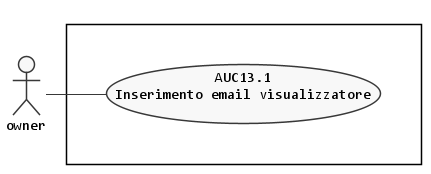
\includegraphics[width=100mm]{aggiunta-visualizzatore.png}
  \caption{AUC9: Aggiunta visualizzatore}%
  \label{fig:AUC9}
\end{figure}

\begin{description}
  \item[Codice:] AUC9;
  \item[Titolo:] Aggiunta visualizzatore;
  \item[Attori primari:] owner;
  \item[Precondizione:] il sistema deve rendere disponibile la pagina di aggiunta visualizzatore;
  \item[Postcondizione:] viene aggiunto il visualizzatore specificato dall'owner;
  \item[Scenario principale:]
  \begin{enumerate}
    \item l'owner vuole aggiungere un visualizzatore alla sua organizzazione.
  \end{enumerate}
\end{description}

\subsubsection{AUC9.1: Inserimento email visualizzatore}%
\label{subs:AUC9.1}
\begin{description}
  \item[Codice:] AUC9.1;
  \item[Titolo:] Inserimento email visualizzatore;
  \item[Attori primari:] owner;
  \item[Precondizione:] il sistema deve rendere disponibile la possibilità di inserire l'email del nuovo visualizzatore;
  \item[Postcondizione:] l'email viene opportunemente inserita;
  \item[Scenario principale:]
  \begin{enumerate}
    \item l'owner inserisce l'email del nuovo visualizzatore.
  \end{enumerate}
\end{description}

\end{document}
